\documentclass[a4paper,12pt]{article}
\usepackage{physics}
\usepackage{amsmath}
\usepackage{amssymb}
\usepackage{graphicx}

\usepackage[hmargin=0.75in,vmargin=0.75in]{geometry}

\title{Inverted Pendulum Mechanics}
\author{Michael Laraia}

\begin{document}

\maketitle



\section{Lagrangian without Drag}

\begin{figure}
    \centering
    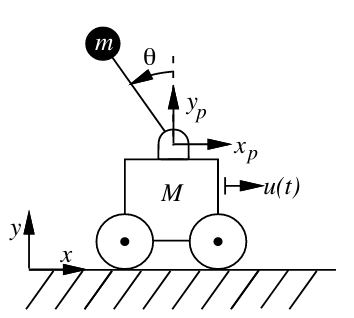
\includegraphics[width=0.6\linewidth]{figs/cartpole2.png}
    \caption{Schematic of an inverted pendulum, and the coordinate system for
    this analysis \cite{cartpole}}
\end{figure}

Lagrangian mechanics can be used to derive the equations of motion of a coupled
system. The Lagrangian $\mathcal{L}$ is defined as
\begin{equation}
    \mathcal{L} = K - U
\end{equation}
where $K$ is kinetic energy, and $U$ is potential energy in the system. For a
driven system, one can encode the driving force $u(t)$ in the Lagrangian
formalism using the concept of virtual work, or using D'alembert's principle.
Virtual work would encode the force in the potential energy via
\begin{equation}
    U = \int u(t) \dot{x} \dd t
\end{equation}

The equations of motion can then be derived from the Lagrangian using the
Euler-Lagrange equation for each state variable $q$
\begin{equation}
    \pdv{\mathcal{L}}{q} = \dv{t} \pdv{\mathcal{L}}{\dot{q}}
\end{equation}

The kinetic energy of the inverted pendulum system is as follows, where $M$ is
the mass of the cart, $m$ is the mass of the ball, $x$ is the position of the
cart, $\theta$ is the counter-clockwise angle of the pole with respect to
vertical, and $l$ is the length of the pole. $g$ is the acceleration due to
gravity.
\begin{align}
    K &= \frac{1}{2} M \dot{x}^2 \nonumber
      + \frac{1}{2} m \qty[ \dot{x} - l \dot{\theta} \cos \theta]^2
      + \frac{1}{2} m \qty(l \dot{\theta} \sin \theta)^2 \\ 
      &= \frac{1}{2} \qty(M+m) \dot{x}^2 + \frac{1}{2} m l^2 \dot{\theta}^2
      - ml \dot{x} \dot{\theta} \cos \theta
\end{align}

The potential energy including virtual work due the driving force is
\begin{equation}
    U = mgl \cos \theta - \int u(t) \dot{x} \dd t
\end{equation}

Then the Lagrangian is
\begin{equation}
    \mathcal{L}
        = \frac{1}{2} \qty(M+m) \dot{x}^2
        + \frac{1}{2} m l^2 \dot{\theta}^2
        - ml \dot{x} \dot{\theta} \cos \theta
        - mgl \cos \theta + \int u(t) \dot{x} \dd t
\end{equation}

The derivatives needed for the Euler-Lagrange equation are listed below
\begin{align*}
    \pdv{\mathcal{L}}{x} &= 0 \\
    %
    \pdv{\mathcal{L}}{\dot{x}} &= (M+m)\dot{x} - ml \dot{\theta} \cos \theta
        - \int u \dd t \\
    %
    \dv{t}\pdv{\mathcal{L}}{\dot{x}} &= 
        (M+m) \ddot{x}
        - ml \ddot{\theta} \cos \theta
        + ml \dot{\theta}^2 \sin\theta
        - u(t) \\
    %
    \pdv{\mathcal{L}}{\theta} &= 
        mgl \sin\theta
        + ml\dot{x} \dot{\theta} \sin\theta \\
    %
    \pdv{\mathcal{L}}{\dot{\theta}} &= 
        ml^2 \dot{\theta} - ml \dot{x} \cos \theta \\
    %
    \dv{t} \pdv{\mathcal{L}}{\dot{\theta}} &= 
        ml^2 \ddot{\theta}^2
        - ml \ddot{x} \cos \theta
        + ml \dot{x}\dot{\theta} \sin \theta
\end{align*}

This results in the following coupled equations for the evolution of the system
\begin{align}
    (M+m) \ddot{x} &= ml \ddot{\theta} \cos \theta
        - ml \dot{\theta}^2 \sin\theta + u(t) \\
    ml^2 \ddot{\theta} &= ml \ddot{x} \cos \theta + mgl\sin\theta
\end{align}

Solving for $\ddot{x}$ and $\ddot{\theta}$ yields:

\begin{align}
    (M+m\sin^2\theta)\ddot{x} &=
        mg\sin\theta \cos\theta - ml\dot{\theta}^2 \sin\theta + u(t) \\
    l(M+m\sin^2\theta) \ddot{\theta} &=
        u(t) \cos\theta - ml\dot{\theta}^2 \sin\theta \cos\theta + (M+m)g\sin\theta
\end{align}

\subsection{Small Angle Approximation}

Suppose we now make the assumption $\theta <<1$, and $\dot{\theta} \approx 0$.
Then $\sin\theta \approx \theta$, and $\cos\theta \approx 1$.

\begin{align*}
    (M+m) \ddot{x} &= ml \ddot{\theta} + u(t) \\
    ml^2 \ddot{\theta} &= ml \ddot{x} + mgl \theta
\end{align*}

\begin{align}
    \ddot{x} &= \frac{mg}{M} \theta + \frac{1}{M} u(t) \\
    %
    \ddot{\theta} &= (m+M)\frac{g}{Ml} \theta + \frac{1}{Ml} u(t)
\end{align}


\subsection{Drag Forces}

Suppose we now include kinetic friction on the cart, and linear air resistance
on the body of the cart. Rolling friction of the cart is described by $F_f =
-\mu_r (M+m)\hat{v}$ with coefficient of kinetic friction $\mu_r$. Drag is
describged by $F_d = -b \vec{v}$, with drag coefficient $b$. We could also
consider quadratic drag $F_q = -c v^2 \hat{v}$, though linear drag dominates
quadratic drag at low velocities.

The Lagrangian becomes:
\begin{align*}
    \mathcal{L} 
        =& \frac{1}{2} \qty(M+m) \dot{x}^2
        + \frac{1}{2} m l^2 \dot{\theta}^2
        - ml \dot{x} \dot{\theta} \cos \theta \\
        &- mgl \cos \theta + \int u(t) \dot{x} \dd t
        + \int \mu_r(M+m)g \dot{x} \dd t
        + \int b \dot{x}^2 \dd t
\end{align*}

The lagrangian derivatives with respect to $\theta$ remain the same, and with
respect to $x$ become:
\begin{align*}
    \pdv{\mathcal{L}}{x} &= 0 \\
    %
    \pdv{\mathcal{L}}{\dot{x}} &= (M+m)\dot{x} - ml \dot{\theta} \cos \theta
        - \int \qty\Big( u - \mu_r(M+m) g - 2b\dot{x} ) \dd t \\
    %
    \dv{t}\pdv{\mathcal{L}}{\dot{x}} &= 
        (M+m) \ddot{x}
        - ml \ddot{\theta} \cos \theta
        + ml \dot{\theta}^2 \sin\theta
        - u(t) + F_f + 2b\dot{x} \\
\end{align*}

Once again applying the Euler-Lagrange equation, we arrive at the following set
of equations governing the system:
\begin{align*}
    (M+m\sin^2\theta) \ddot{x} &= mg \sin\theta\cos\theta
        - ml\dot{\theta}^2\sin\theta
        + u(t)
        - \mu_r(M+m)g
        - 2b\dot{x} \\
    l (M + m\sin^2\theta) \ddot{\theta} &= u(t) \cos\theta
        - ml \dot{\theta}^2 \sin\theta \cos\theta
        + (M+m)g\sin\theta \\
        &- \mu_r(M+m) \cos\theta
        - 2b\dot{x} \cos\theta
\end{align*}

We can once again use the small angle approximation:
\begin{align}
    (M+m) \ddot{x} &= mg\theta + u(t) - \mu_r(M+m)g - 2b\dot{x} \\
    %
    ml^2\ddot{\theta} &= ml\ddot{x} + mgl\theta
\end{align}

\begin{align}
    \ddot{x} &= \frac{mg}{M}\theta + \frac{1}{M} u(t) - \frac{\mu(M+m)}{M}g
        - \frac{2b}{M}\dot{x} \\
    %
    \ddot{\theta} &= \qty[\frac{mg}{Ml} + \frac{g}{l}]\theta
        + \frac{1}{Ml} \qty[ u(t) - \mu(M+m)g - 2b\dot{x}]
\end{align}

\end{document}
